% !TEX root = ../CategoricalCoDesign.tex
\section{Concepts of  Formal Engineering Design}
This section introduces the basic concepts of engineering design, and describes the questions we want to answer with our work.

\subsection{Basic concepts of formal engineering design}
We will informally introduce some of the basic nomenclature of engineering
design~\cite{book-formal-engineering-design}. Later, all these concepts will find a formal
definition in the language of category theory.

\paragraph{Functionality and functional requirements}
You are an engineer in front of an empty whiteboard, ready to start designing the next product.
The first question to ask is: What is the \emph{purpose} of the product to be designed? The purpose of the product is expressed by the \emph{functional requirements}, sometimes called
\emph{functional specifications}, or simply \emph{function}.

Unfortunately, the word ``function'' conflicts with the mathematical concept. Therefore, we
will talk  about \emph{functionality}. Moreover, we will never use the word ``function'', and
instead use \emph{map} to denote the mathematical concept.

\begin{example}
    These are a few examples of functional requirements:

    \begin{compactitem}
        \item A car must be able to transport at least $n \geq 4$ passengers.
        \item A battery must store at least $\unit[100]{kJ}$ of energy.
        \item An autonomous vehicle should reach at least $\unit[20]{mph}$ while guaranteeing safety.
    \end{compactitem}
\end{example}

\paragraph{Resources and resource constraints}

We call \emph{resources} what we need to pay to realize the given functionality.
In some contexts, these are better called \emph{costs}, or \emph{dependencies}.


\begin{example}
These are a few examples of resource constraints:
\begin{compactitem}
\item A car should not cost more than \unit[15,000]{USD}.
\item A battery should not weigh more than \unit[1]{kg}.
\item A process should not take more than \unit[10]{s}.
\end{compactitem}
\end{example}

\paragraph{Duality of functionality and resources}

There is an interesting duality between functionality and resources. When designing systems, one is given functional requirements, as a \emph{lower bound} on the
functionality to provide, and one is given resource constraints, which are an \emph{upper bound} on the
resources to use.

As far as design objectives go, most can be understood as either \emph{minimize resource usage}
or \emph{maximize functionality provided}.

This duality between functionality and resources will be at the
center of our formalization.

\paragraph{Non-functional requirements}

Functionality and resources do not cover all the requirements--- there is, for example, a
large class of \emph{non-functional requirements}~\cite{??} such as the extensibility and the
maintainability of the system. Nevertheless, functionality and resources can express most of
the requirements which can be quantitatively evaluated, at least prior to designing, assembling,
and testing the entire system.

\paragraph{Implementation space}

The \emph{implementation space} or \textit{design space} is the set of all possible design choices that could be chosen;
by \textit{implementation}, or the word ``design'', used as a noun, we mean one particular  set of choices. The implementation space $I$ is the set over which we are optimizing; an implementation $i\in I$ is a particular point in that set~(\cref{fig:impspace}).

\begin{figure}[h!]
    \begin{center}
    \includesag{15_imp_space}
    \end{center}
    \caption{An \emph{implementation} $i$ is a particular point in the implementation space $I$.}
    \label{fig:impspace}
\end{figure}


The interconnection between functionality, resources, and implementation spaces
is as follows. We will assume that, given one implementation, we can evaluate it
to know the functionality and the resources spaces~(\cref{fig:FIR}).

\begin{figure}[h!]
    \centering
    \includesag{30_dpcatfig_fir}
    %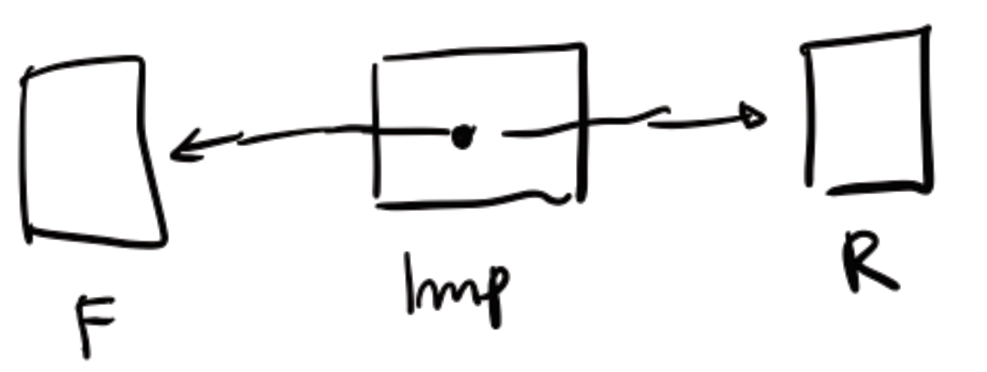
\includegraphics[scale=0.33]{dpcatfig_fir}
    \caption{Evaluation of specific implementations to get functionality and resources spaces.\label{fig:FIR}}
\end{figure}

\paragraph{Systems and components}

Engineers tend to approach complex design problems hierarchically.  The usual
nomenclature refers to \textit{systems} being decomposed into \textit{components}.

\noindent What is a system, and what is a component? Here is a great quote:

\begin{quote}
A system is composed of components; \\
a component is something you understand.\\
---Howard Aiken\footnote{
Howard H. Aiken (1900-1973), creator of the MARK I computer.
Quoted by Kenneth E. Iverson (1920-2004), creator of programming language APL.
Quoted in this paper\cite{that-paper},
  but ultimately sourceless and probably apocryphal.}
\end{quote}

The first part of the quote, "A system is composed of components", is plain as day as much as
it is tautological. We could equally say: "A system is partitioned in parts".

The second part, "a component is something you understand", is the insightful part: We call
"system" what is not obvious to understand, even if we understand all its components
separately.

Whether something can be considered a component, an indivisible atom in the theory, depends on the context.
%
% This definition is, of course, an anthropocentric definition, as it is a
% limitation of the human mind, related to the amount of neurons in the brain. It
% also depends on what exactly is the task at hand with which we are confronted.


\paragraph{Interfaces and interconnection}

Components are \emph{interconnected} to create a system.
This implies that we have defined the \emph{interfaces} of components, which
have the dual function of delimiting when one component ends and another begins,
and also to describe exactly what is the nature of their interaction.

In this paper, we will present a formalism in which the functionality and resources
are the interfaces used for interconnection: Two components are connected
if the resources required by the first correspond to the functionality
provided by the second.




\paragraph{Abstraction}

By \emph{abstraction}, one usually means that it is possible to ``zoom out'',
in the sense that a system of components can be seen as a component itself,
which can be part of larger systems.


\paragraph{Compositionality}

A \emph{compositional} property is a property that is preserved by interconnection and abstraction; assuming each component in a system satisfies that property, also the system as a whole satisfies the property.

\begin{example}
One can compose two electronic circuits by joining their terminals to obtain
another electronic circuit. We would say that the property
of being an electronic circuit is compositional.
\end{example}



\subsection{Queries in design}

\paragraph{Design Queries} The design queries we will present throughout this paper are the following:
\begin{compactitem}
\item Given a certain functionality, find the minimal resources that can realize it, or provide a proof that there are none.
\item Given certain resources, find the maximal functionality that can be realized, or provide a proof that there are none.
\item \todo{...} 
\end{compactitem}



